% !TEX root = ../BookTemplate.tex
%%%%%%%%%%%%%%%%%%%%%%%%%%%%%%%%%%%%%%%%%%%%%%%%%%%%%%%%%%%%%%%%%%%%%%%%%%%%%%%%%%
\chapter{ทฤษฎีการจำลองสถานการณ์ (Simulation)}

\section*{โจทย์ธุรกิจ: ความไม่แน่นอนในกระบวนการผลิตของ ABC Furniture}

\begin{tcolorbox}[colback=white!100!white, colframe=black!80!white,
  title=ข้อความจากคุณสมชาย,
  fonttitle=\bfseries,
  sharp corners=southwest,
  boxrule=0.8pt,
  left=1mm, right=1mm, top=1mm, bottom=1mm,
]
\emph{
"หลังจากที่เราได้วางแผนการผลิตและกลยุทธ์รับมือกับตลาดที่ไม่แน่นอนผ่านแบบจำลองเชิงเส้นและทฤษฎีการตัดสินใจเรียบร้อยแล้ว  
แต่สิ่งที่เรายังไม่สามารถคาดการณ์ได้แน่นอน คือเวลาที่ต้องใช้ในแต่ละขั้นตอนของกระบวนการผลิตจริง ๆ  
บางครั้งแรงงานลาป่วย บางครั้งเครื่องจักรเสีย หรือบางสัปดาห์มีคำสั่งซื้อเร่งด่วนแทรกเข้ามา  
เราจึงอยากจำลองสถานการณ์เหล่านี้ เพื่อดูว่าจะกระทบต่อการผลิตและการจัดส่งอย่างไร และควรจะปรับการจัดการโรงงานอย่างไรดี"
}
\end{tcolorbox}

บริษัท ABC Furniture กำลังเผชิญกับความไม่แน่นอนใน \textbf{ระยะเวลาการผลิตแต่ละชิ้นงาน} และ \textbf{ปริมาณคำสั่งซื้อที่เปลี่ยนแปลงตลอดเวลา} โดยเฉพาะในช่วงโปรโมชั่นและเทศกาลยอดนิยม ซึ่งอาจทำให้กระบวนการผลิตไม่สามารถดำเนินไปตามแผนได้

เพื่อรองรับเหตุการณ์ที่คาดเดาไม่ได้เหล่านี้ ผู้จัดการฝ่ายผลิตต้องการเครื่องมือในการ “ทดลอง” และ “คาดการณ์ผลลัพธ์” ของทางเลือกที่เป็นไปได้ โดยไม่ต้องเสี่ยงจริงในโลกธุรกิจจริง ซึ่งนำไปสู่แนวคิดของ \textbf{การจำลองสถานการณ์ (Simulation)} ที่จะช่วยให้บริษัทสามารถวิเคราะห์ผลกระทบจากตัวแปรสุ่มต่าง ๆ ต่อกระบวนการผลิตได้อย่างมีประสิทธิภาพ

\bigskip

\noindent\textbf{คำถามชวนคิด:}
\begin{itemize}
    \item ในสถานการณ์แบบนี้ คุณคิดว่า “สูตรคำนวณตายตัว” ที่เคยใช้ในบทก่อน ๆ ยังเหมาะสมอยู่หรือไม่?
    \item คุณจะเก็บข้อมูลอะไรเพื่อใช้ในการจำลองเหตุการณ์ในกระบวนการผลิต?
    \item คุณจะจำลองขั้นตอนใดในกระบวนการผลิตก่อน เช่น เวลาในการประกอบสินค้า การขนส่ง หรือการเตรียมวัตถุดิบ?
    \item ถ้าคุณลอง “สุ่มเหตุการณ์” ต่าง ๆ แล้วพบว่าเกิดความล่าช้าเป็นประจำ คุณจะวางแผนการผลิตใหม่อย่างไร?
    \item ถ้าต้องเขียนโปรแกรมจำลองขั้นตอนการผลิต คุณจะออกแบบลำดับเหตุการณ์หรือเงื่อนไขไว้อย่างไร?
    \item ผลลัพธ์ของการจำลองแบบใดที่จะช่วยให้ฝ่ายผลิตวางแผนจัดกำลังคนและเครื่องจักรได้ดีขึ้น?
\end{itemize}

\newpage
\section{แนวคิดเบื้องต้นของการจำลอง}
\begin{itemize}
    \item บางสถานการณ์อาจไม่สามารถเขียนสมการทางคณิตศาสตร์ตัวแบบเพื่ออธิบายสถานการณ์ได้เพราะระบบมีความซับซ้อนมากเกินไปหรือมีเงื่อนไขบางประการที่ทำให้ไม่สามารถใช้ตัวแบบที่มีอยู่แล้วได้
    \item ทำให้ต้องสุ่มภายใต้ข้อมูลที่มีเพื่อประมาณค่าจากการทำการทดลองสุ่มหลาย ๆ การทดลอง
    \item ในหัวข้อกรณีตัวอย่างที่จะกล่าวถึงถัดไป เป็นตัวอย่างพื้นฐานที่แสดงให้เห็นว่าการทำการทดลองสุ่มโดยที่จำลองสถานการณ์ให้เหมือน (หรือคล้าย) เหตุการณ์จริงจะสามารถประมาณค่าผลเฉลยให้ใกล้เคียงค่าจริงได้
\end{itemize}

\subsection{กรณีตัวอย่าง: การหาค่า $\pi$}
จากชุดความรู้เบื้องต้นที่เรามีคือ $\pi= \frac{\pi r^2}{r^2} = \frac{4\pi r^2}{(2r)^2} =4 \left( \frac{\text{พื้นที่วงกลม}}{\text{พื้นที่สี่เหลี่ยมจตุรัสที่แนบวงกลม}}\right)$
\begin{center}
\begin{tikzpicture}[scale=2]
  % Square
  \draw[thick] (-1,-1) rectangle (1,1);
  \node at (1.1,1.1) {$2r$};

  % Circle
  \draw[thick, fill=blue!10] (0,0) circle(1);
  \node at (0.6,0.2) {\small พื้นที่วงกลม = $\pi r^2$};

  % Square area label
  \node at (0,-1.3) {\small พื้นที่สี่เหลี่ยม = $(2r)^2 = 4r^2$};

  % Radius line
  \draw[->, thick, red] (0,0) -- (1,0) node[midway, below] {$r$};
\end{tikzpicture}
\end{center}
แต่เราไม่รู้ว่าค่า $\pi$ คือเท่าไหร่ เราจึงออกแบบการทดลองที่ถูกออกแบบให้อธิบายชุดความรู้ที่เรามีได้ ซึ่งก็คือการสุ่มโยนจุดเข้าไปในรูปสี่เหลี่ยม แล้วหาอัตราส่วนของจำนวนจุดที่อยู่ภายในวงกลม (แสดงถึงพื้นที่วงกลม) ต่อจำนวนจุดทั้งหมดที่โยนเข้าไป (แสดงถึงพื้นที่สี่เหลี่ยมจัตุรัส) แล้วนำอัตราส่วนที่ได้มาคูณกับ 4 จะได้ค่าประมาณของ $\pi$

เพื่อให้การสุ่มสามารถถูกควบคุมและวัดผลได้ เราจึงต้องใช้ระบบพิกัดฉากเข้ามาช่วยในการแสดงผล โดยที่เราจะให้จุดศูนย์กลางของวงกลมวางที่จุดกำเนิด และรัศมีของวงกลมมีค่าเท่ากับ $r=1$
\begin{center}
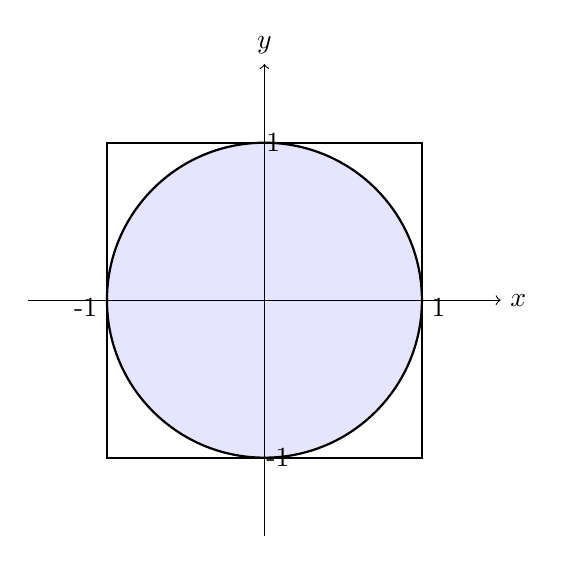
\begin{tikzpicture}[scale=2]
  % แกน x และ y
  % วงกลม
  \draw[thick, fill=blue!10] (0,0) circle(1);
  
  \draw[->] (-1.5,0) -- (1.5,0) node[right] {$x$};
  \draw[->] (0,-1.5) -- (0,1.5) node[above] {$y$};

  \draw (1,0.05) -- (1,-0.05) node[right] {1};
  \draw (-1,0.05) -- (-1,-0.05) node[left] {-1};
  \draw (0.05,1) -- (-0.05,1) node[right] {1};
  \draw (0.05,-1) -- (-0.05,-1) node[right] {-1};

  % สี่เหลี่ยมจัตุรัส
  \draw[thick] (-1,-1) rectangle (1,1);
\end{tikzpicture}
\end{center}
และเงื่อนไขการสุ่มจุด $(x,y)$ เป็นไปดังนี้
\begin{itemize}
    \item การสุ่มเป็นแบบ uniform กล่าวคือทุุกตำแหน่งมีโอกาสเท่ากัน
    \item สุ่ม $x$ และ $y$ อยู่ในช่วง $[-1,1]$ เพื่อให้มั่นใจว่าอยู่ภายในสี่เหลี่ยมจตุรัส
\end{itemize}
ทั้งนี้ การตรวจสอบว่าจุด $(x,y)$ อยู่ในวงกลมหรือไม่ เราสามารถเช็คได้ด้วยเงื่อนไขว่า
$$
x^2 + y^2 \leq 1
$$
ซึ่งเราสามารถใช้ Excel ช่วยในการสุ่มได้ดังนี้
\begin{itemize}
    \item Column A: ครั้งที่ทดลอง
    \item Column B-C: สุ่ม $x$ และ $y$ ด้วยคำสั่ง =RANDARRAY(จำนวนครั้งที่ทดลอง,2,-1,1,FALSE)
    \item Column D: เช็คว่าจุดอยู่ในวงกลมหรือไม่โดยใช้ ColumnB$\textasciicircum$2 + ColumnC$\textasciicircum$2 <= 1
    \item Column E: นับจำนวนจุดที่อยู่ในวงกลมตั้งแต่การทดลองที่ 1 จนถึงการทดลองปัจจุบัน
    \item Column F: หาค่า 4*อัตราส่วน
\end{itemize}
ตัวอย่าง 5 แถวแรกและ 5 แถวสุดท้ายของตารางกรณีสุ่ม 30000 ครั้ง:
\begin{center}
    \includegraphics[width=0.7\linewidth]{image.png}
    \includegraphics[width=0.7\linewidth]{image2.png}
\end{center}
และเมื่อลองทำการพล็อตกราฟของค่าที่เราสนใจ (Column F) จะได้ดังรูป
\begin{center}
    \includegraphics[width=\linewidth]{ratioToPi.png}
\end{center}
ซึ่งจะเห็นว่ายิ่งเราทำการสุ่มมากขึ้นเท่าไหร่ ค่าที่เราตั้งไว้ (4 เท่าของอัตราส่วน) เพื่อวัดสิ่งที่เราอยากค้นหา (ค่า $\pi$) จะยิ่งเข้าใกล้ค่าที่เราอยากค้นหาดังกล่าวมากขึ้นเรื่อยๆ

สามารถออกแบบการทดลองในทำนองเดียวกันคือทำการทดลองสุ่ม 30000 จุดหลาย ๆ รอบแล้วหาค่าเฉลี่ยค่าของรอบสุ่มที่ 30000 ของทุกชุดการทดลองก็ได้เช่นกันโดยรูปด้านล่างคือตัวอย่างการทดลองที่ทำการทดลอง 500 รอบ ซึ่งได้ค่าเฉลี่ยของค่าอัตราส่วนรอบที่ 30000 อยู่ที่ 3.141638 จากค่าประมาณจริง ๆ ของ $\pi\approx 3.1415926$ (ถ้าทำใน Excel อาจจะเจอปัญหาเรื่อง memory ไม่พอ แต่จะมีความแม่นยำกว่าการทดลองรอบเดียว เลยอาจต้องใช้เครื่องมือเช่นเขียน Python)
\begin{center}
    \includegraphics[width=1\linewidth]{SimulatePi.png}
\end{center}

ทั้งนี้ จะเห็นว่าเรามีการกำหนดเงื่อนไขการสุ่ม ซึ่งเป็นสิ่งที่สำคัญที่สุดของการจะจำลองสถานการณ์ ตัวอย่างเช่นกรณีนี้ก็คือต้องสุ่มแบบ Uniform เนื่องจากลักษณะการคำนวณอัตราส่วนของพื้นที่นั้นมีสมมติฐานว่าทุกจุดพื้นที่จะต้องมีความสำคัญเท่ากัน ไม่มีจุดใดจุดหนึ่งที่มีโอกาสมากกว่าจุดอื่นเพื่อไม่ให้เกิดอคติ (bias) ในการสุ่ม เช่นในตัวอย่างเดิม ถ้าเราเปลี่ยนสมมติฐานตั้งต้นให้สุ่มแบบ Normal Distribution ที่มีค่าเฉลี่ยเป็น 0 และส่วนเบี่ยงเบนมาตรฐานที่ 0.3 ที่จะมีโอกาสสุ่มได้บริเวณจุดกำเนิดมากกว่าจุดขอบ ๆ ซึ่งจะแสดงพฤติกรรมว่าจุดนอกวงกลมมีโอกาสน้อยกว่าจุดในวงกลม จะได้ว่าผลการประมาณค่าเปลี่ยนเป็น 3.9844 แทนที่จะเข้าใกล้ค่า $\pi$ ตามรูป
\begin{center}
    \includegraphics[width=1\linewidth]{simulatePiWrong.png}
\end{center}

\begin{tcolorbox}[colback=white!100!white, colframe=black!80!white,
  title=หมายเหตุ (สำหรับอ่านเพิ่มเติม),
  fonttitle=\bfseries,
  sharp corners=southwest,
  boxrule=0.8pt,
  left=1mm, right=1mm, top=1mm, bottom=1mm, breakable
]
    ตัวอย่างนี้เป็นตัวอย่างที่มีทฤษฎีเบื้องหลังและสามารถพิสูจน์ทางคณิตศาสตร์เพื่อยืนยันว่าผลที่ได้จากการทดลองเป็นไปตามทฤษฎี (อาจมีคลาดเคลื่อนเล็กน้อย) เนื่องจากเป็นสถานการณ์ที่สามารถอธิบายได้ด้วยการแจกแจงความน่าจะเป็นที่ไม่ซับซ้อน (ซึ่งไม่ค่อยพบในโลกจริงที่มักจะเป็นระบบที่ซับซ้อน)
    \newpage
    \textbf{กรณีที่ $X, Y$ แจกแจงแบบคงที่}
    \begin{proof}
        กำหนดให้ $X, Y$ เป็นตัวแปรสุ่มอิสระ ซึ่งแจกแจงแบบสม่ำเสมอ (Uniform) บนช่วง $[-1, 1]$ ดังนั้นคู่ $(X, Y)$ จะกระจายอยู่ทั่วพื้นที่ของสี่เหลี่ยมจัตุรัสที่มีด้านยาว 2 หน่วย และมีพื้นที่รวมเท่ากับ $4$ หน่วยตาราง

        นิยามเหตุการณ์ $A$ ว่าเป็นเหตุการณ์ที่จุด $(X, Y)$ ตกอยู่ภายในวงกลมรัศมี 1 ซึ่งมีสมการคือ $X^2 + Y^2 \leq 1$

        จะได้ว่า
        \[
            P((X, Y) \in A) = \frac{\text{พื้นที่ของวงกลม}}{\text{พื้นที่ของสี่เหลี่ยมจัตุรัส}} = \frac{\pi \cdot 1^2}{4} = \frac{\pi}{4}
        \]

        เมื่อสุ่มจุด $N$ จุดจากการแจกแจงนี้ ให้ $S$ เป็นจำนวนจุดที่ตกในวงกลม จะได้ว่า $S = \sum_{i=1}^N \mathbf{1}_{(X_i, Y_i) \in A}$

        ดังนั้นสัดส่วนของจุดที่อยู่ในวงกลมคือ $Z = \frac{S}{N}$ ซึ่งเป็นตัวแปรสุ่ม และค่าคาดหมายคือ:
        \[
            \mathbb{E}\left[Z\right] =\mathbb{E}\left[\frac{S}{N}\right] = \frac{1}{N} \sum_{i=1}^N \mathbb{E}\left[\mathbf{1}_{(X_i, Y_i) \in A}\right] = P((X, Y) \in A) = \frac{\pi}{4}
        \]

        นั่นคือ ค่าคาดหวังของสัดส่วนของจุดที่อยู่ในวงกลมจะมีค่าเท่ากับ $\frac{\pi}{4}$ เสมอ โดยไม่ขึ้นกับจำนวนจุด $N$
    \end{proof}
    \vspace{1em}

    \textbf{กรณีที่ $X, Y \sim \mathcal{N}(0, 0.09)$} (ค่าความเบี่ยงเบนมาตรฐาน $\sigma = 0.3$)
    \begin{proof}
        เนื่องจากบทพิสูจน์ในส่วนของตัวแปรสุ่ม $Z$ ไม่ขึ้นกับการแจกแจงของตัวแปรสุ่ม $X,Y$ ดังนั้น เราจึงยังสามารถได้ผลว่า
        \[
            \mathbb{E}\left[Z\right] =\mathbb{E}\left[\frac{S}{N}\right] = P((X, Y) \in A)
        \]
        เหลือแค่หาค่าความน่าจะเป็น $P((X, Y) \in A) = P(X^2 + Y^2 \leq 1)$ พิจารณาตัวแปรสุ่ม $R^2=X^2 + Y^2$ ซึ่งจากนิยามของการแจกแจง Chi-square (ผลรวมกำลังสองของตัวแปรสุ่มที่มีการแจกแจงปกติมาตรฐาน) จะได้ว่า
        $$
        \frac{R^2}{0.09}=\frac{X^2 + Y^2}{\sigma^2} = \left( \frac{X}{\sigma} \right)^2 + \left( \frac{Y}{\sigma} \right)^2 \sim \chi^2(2)
        $$
        ดังนั้น $P(R^2 \leq 1) = P(\chi^2(2) \leq \frac{1}{0.09}) = 1-\exp{-\frac{1}{2\times 0.09}}$\\
        เพราะฉะนั้น $E[4Z] = 4P(R^2\leq 1) = 4\left( 1-\exp{-\frac{1}{2\times 0.09}}\right)\approx 3.9845$
    \end{proof}
\end{tcolorbox}


\newpage
\section{ตัวแบบและขั้นตอนการจำลองสถานการณ์ (Simulation Process)}

จากตัวอย่างที่แล้ว เราได้เห็นกระบวนการที่สำคัญของการจำลองสถานการณ์ (Simulation) ซึ่งประกอบไปด้วยขั้นตอนหลัก ๆ ตั้งแต่การกำหนดวัตถุประสงค์, การเก็บข้อมูล, การเลือกตัวแบบ, การสุ่มตัวอย่าง และการวิเคราะห์ผลลัพธ์ที่ได้จากการทดลอง ในหัวข้อนี้เราจะสรุปขั้นตอนที่จำเป็นทั้งหมดในการจำลองสถานการณ์ทั่วไป ซึ่งสามารถนำไปประยุกต์ใช้กับสถานการณ์ทางธุรกิจต่าง ๆ ได้อย่างเป็นระบบ

กระบวนการในการจำลองสถานการณ์ประกอบด้วยขั้นตอนที่สำคัญ ดังนี้:

\begin{enumerate}
    \item \textbf{กำหนดวัตถุประสงค์ของการจำลอง (Define Simulation Objective)}\\
    ขั้นตอนแรกคือการระบุให้ชัดเจนว่าการจำลองครั้งนี้มีเป้าหมายอะไร เช่น บริษัท ABC Furniture ต้องการจำลองระยะเวลาในการผลิตสินค้าเพื่อดูว่าจะส่งผลต่อการส่งมอบสินค้าได้ทันตามกำหนดหรือไม่
    
    \item \textbf{กำหนดตัวแบบและตัวแปรที่เกี่ยวข้อง (Identify the Model and Relevant Variables)}\\
    หลังจากรู้วัตถุประสงค์แล้ว เราต้องกำหนดว่าอะไรคือสิ่งที่เราจะจำลอง ในทางธุรกิจอาจมีตัวแปรเช่น เวลามาถึงของลูกค้า, ระยะเวลาการผลิตสินค้า, ระยะเวลาการให้บริการ, หรือแม้กระทั่งปริมาณความต้องการของตลาดในแต่ละช่วงเวลา เป็นต้น
    
    \item \textbf{เก็บรวบรวมข้อมูลจากระบบจริง (Data Collection)}\\
    เมื่อระบุตัวแปรที่เกี่ยวข้องแล้ว ขั้นตอนถัดไปคือการเก็บข้อมูลเพื่อระบุลักษณะทางสถิติของตัวแปรนั้น ๆ เช่น การเก็บข้อมูลเวลาการผลิตจริงย้อนหลังหลายสัปดาห์ หรือข้อมูลพฤติกรรมของลูกค้าที่เกิดขึ้นจริงในอดีต
    
    \item \textbf{เลือกและสร้างแบบจำลองความน่าจะเป็น (Select and Build Probability Models)}\\
    หลังจากเก็บข้อมูล เราจึงนำข้อมูลนั้นมาวิเคราะห์เพื่อระบุการแจกแจงความน่าจะเป็นที่เหมาะสม เช่น เวลาการผลิตอาจเป็นแบบ Normal หรือ Exponential, จำนวนลูกค้าที่เข้าร้านอาจมีการแจกแจงแบบ Poisson หรือแบบ Uniform ดังในตัวอย่างที่ผ่านมาที่เราใช้ Uniform ในการประมาณค่า $\pi$
    
    \item \textbf{กำหนดเงื่อนไขการสุ่มและกฎของระบบ (Define Randomness Conditions and System Rules)}\\
    ขั้นตอนนี้คือการออกแบบกลไกของการจำลอง เช่น จะสุ่มตัวแปรต่าง ๆ อย่างไร ต้องใช้เครื่องมืออะไร มีเงื่อนไขและข้อจำกัดของระบบอย่างไรบ้าง เช่น บริษัท ABC Furniture อาจตั้งเงื่อนไขว่าหากการผลิตล่าช้ากว่าเวลาที่กำหนด จะส่งผลต่อกำหนดการจัดส่งสินค้าอย่างไร เป็นต้น
    
    \item \textbf{ดำเนินการจำลองสถานการณ์ (Perform Simulation Runs)}\\
    เมื่อโมเดลพร้อมแล้ว จะต้องดำเนินการจำลองซ้ำหลายครั้ง (replications) เพื่อให้ได้ผลลัพธ์ที่สะท้อนพฤติกรรมระบบจริงอย่างถูกต้องชัดเจน โดยอาจดำเนินการซ้ำหลายร้อยหรือหลายพันครั้งขึ้นอยู่กับลักษณะของปัญหา
    
    \item \textbf{วิเคราะห์ผลลัพธ์ที่ได้จากการจำลอง (Analyze Simulation Results)}\\
    หลังจากที่ทำการทดลองจำลองซ้ำหลาย ๆ รอบแล้ว เราจะนำผลลัพธ์ที่ได้มาวิเคราะห์เชิงสถิติ เช่น การหาค่าเฉลี่ย, ส่วนเบี่ยงเบนมาตรฐาน, ความน่าจะเป็นของเหตุการณ์ที่สนใจ เช่น โอกาสที่สินค้าไม่สามารถส่งมอบทันเวลา หรือเวลารอคอยเฉลี่ยของลูกค้า เป็นต้น
    
    \item \textbf{ตรวจสอบความถูกต้องและความแม่นยำของตัวแบบ (Validate and Verify the Model)}\\
    ก่อนนำไปใช้งานจริง เราต้องตรวจสอบว่าผลลัพธ์จากแบบจำลองนั้นตรงกับสิ่งที่เกิดขึ้นในระบบจริงมากแค่ไหน หากผลที่ได้จากตัวแบบมีความคลาดเคลื่อนสูง เราต้องกลับไปตรวจสอบข้อมูลหรือโมเดลที่ใช้ใหม่
    
    \item \textbf{การนำผลลัพธ์ไปประยุกต์ใช้ในทางปฏิบัติ (Implementation and Decision Making)}\\
    ขั้นตอนสุดท้ายคือการนำผลที่ได้จาก Simulation ไปใช้ในการตัดสินใจจริงในธุรกิจ เช่น บริษัท ABC Furniture อาจนำผลการจำลองไปกำหนดแผนการผลิตและจัดการทรัพยากรใหม่เพื่อลดความเสี่ยงในการผลิตและเพิ่มประสิทธิภาพของระบบ
\end{enumerate}

กระบวนการทั้งหมดนี้สามารถสรุปออกมาในลักษณะของแผนภาพดังนี้

\begin{center}
    \begin{tikzpicture}[node distance=1.5cm,auto,font=\small]
        \node[draw, rounded corners, fill=blue!10] (start) {กำหนดวัตถุประสงค์};
        \node[draw, rounded corners, fill=blue!10, below of=start] (identify) {กำหนดตัวแปรที่เกี่ยวข้อง};
        \node[draw, rounded corners, fill=blue!10, below of=identify] (collect) {เก็บข้อมูลจากระบบจริง};
        \node[draw, rounded corners, fill=blue!10, below of=collect] (prob) {เลือกและสร้างแบบจำลองความน่าจะเป็น};
        \node[draw, rounded corners, fill=blue!10, below of=prob] (rules) {กำหนดเงื่อนไขการสุ่มและกฎของระบบ};
        \node[draw, rounded corners, fill=blue!10, below of=rules] (simu) {ดำเนินการจำลอง};
        \node[draw, rounded corners, fill=blue!10, below of=simu] (analyze) {วิเคราะห์ผลลัพธ์};
        \node[draw, rounded corners, fill=blue!10, below of=analyze] (validate) {ตรวจสอบความถูกต้อง};
        \node[draw, rounded corners, fill=blue!10, below of=validate] (implement) {นำไปใช้ในการตัดสินใจ};

        \draw[->, thick] (start) -- (identify);
        \draw[->, thick] (identify) -- (collect);
        \draw[->, thick] (collect) -- (prob);
        \draw[->, thick] (prob) -- (rules);
        \draw[->, thick] (rules) -- (simu);
        \draw[->, thick] (simu) -- (analyze);
        \draw[->, thick] (analyze) -- (validate);
        \draw[->, thick] (validate) -- (implement);
    \end{tikzpicture}
\end{center}

โดยในหัวข้อถัดไป เราจะศึกษาและเจาะลึกเทคนิคการสุ่มแบบ Monte Carlo ซึ่งเป็นหัวใจสำคัญของกระบวนการจำลองสถานการณ์ในธุรกิจ เพื่อให้เห็นภาพการประยุกต์ใช้กระบวนการจำลองได้อย่างเป็นระบบยิ่งขึ้น

\section{การสุ่มตัวอย่างแบบ Monte Carlo ในการจำลองสถานการณ์ในธุรกิจ}
\textbf{การจำลองแบบมอนติคาร์โล} (Monte Carlo Simulation) เป็นเทคนิคที่ใช้วิธีการสุ่มตัวแปรเข้ามาช่วยในการประเมินผลลัพธ์ที่อาจเกิดขึ้นภายใต้สภาวะที่ไม่แน่นอน เทคนิคนี้มีรากฐานจากแนวคิดในทฤษฎีความน่าจะเป็นและสถิติ โดยเฉพาะอย่างยิ่งเมื่อปัญหาที่ต้องการศึกษามีความซับซ้อนเกินกว่าจะหาคำตอบได้ด้วยวิธีวิเคราะห์เชิงพีชคณิตแบบตรง

แก่นของมอนติคาร์โลคือการ “สุ่มค่าตัวแปรตามการแจกแจงที่กำหนด” เพื่อนำไปแทนค่าในโมเดล แล้วคำนวณผลลัพธ์ที่เกิดขึ้น จากนั้นทำซ้ำการสุ่มจำนวนมากเพื่อดูพฤติกรรมรวมของผลลัพธ์ เช่น ค่าคาดหมาย ค่ามากสุด ค่าน้อยสุด หรือค่าที่อยู่ในช่วงความเชื่อมั่นที่กำหนด โดยตัวอย่างการแจกแจงที่นิยมใช้งานกันอยู่แล้วมีดังนี้
\begin{itemize}
    \item ถ้าค่าใช้จ่ายในอนาคตมีความไม่แน่นอน อาจสุ่มค่าใช้จ่ายจากการแจกแจง Normal หรือ Triangular
    \item ถ้าความต้องการสินค้าในอนาคตขึ้นอยู่กับพฤติกรรมผู้บริโภค อาจสุ่มจำนวนจากการแจกแจง Poisson
    \item ถ้าความสำเร็จของกระบวนการหรือขั้นตอนมีแค่ 2 ผลลัพธ์ (สำเร็จ/ล้มเหลว ในภาษาของการแจกแจงความน่าจะเป็น) อาจใช้การแจกแจงแบบ Bernoulli หรือ Binomial
    \item ถ้าจำนวนลูกค้าในช่วงเวลาหนึ่งมีความแปรผัน อาจใช้การแจกแจง Poisson เพื่อสุ่มจำนวนลูกค้า
    \item ถ้าเวลาระหว่างลูกค้ารายถัดไปมีลักษณะสุ่มและต่อเนื่อง อาจใช้การแจกแจง Exponential เพื่อสุ่มระยะเวลาการรอลูกค้าเข้าร้าน
\end{itemize}
ซึ่งเป็นขั้นตอนที่สำคัญมาก ๆ และการเก็บข้อมูลและลายละเอียดพฤติกรรมทางธุรกิจให้ละเอียดพอจะช่วยทำให้เราเลือกการแจกแจงของตัวแปรได้แม่นยำและใกล้เคียงความเป็นจริงได้ (อาจจะใช้เรื่องการทำ goodness of fit test มาช่วยตรวจสอบในขั้นตอนการตรวจสอบได้)

\subsection*{5 ขั้นตอนการทำ Monte Carol Simulation}
\begin{enumerate}
    \item \textbf{กำหนดการแจกแจงความน่าจะเป็นของตัวแปรสำคัญ} \\
    ระบุ \textit{ตัวแปรสำคัญ} ที่ต้องการจำลอง เช่น ความต้องการสินค้า เวลารอ จำนวนลูกค้าในแต่ละวัน ฯลฯ จากนั้นคำนวณ \textit{ความน่าจะเป็น} โดยใช้ข้อมูลในอดีต เช่น ความถี่ของแต่ละเหตุการณ์หารด้วยความถี่รวมทั้งหมด
    
    \item \textbf{สร้างการแจกแจงความน่าจะเป็นสะสม (Cumulative Probability)} \\
    สร้างคอลัมน์ความน่าจะเป็นสะสม โดยการบวกค่าความน่าจะเป็นในข้อก่อนหน้าแบบสะสมต่อเนื่อง เพื่อใช้เป็นขอบเขตในการแมปกับช่วงของเลขสุ่ม
    
    \item \textbf{กำหนดช่วงของเลขสุ่ม (Random Number Interval)} \\
    แปลงความน่าจะเป็นสะสมให้เป็นช่วงของเลขสุ่ม เช่น 00--99 หรือ 000--999 โดยการจับคู่ค่าที่เป็นไปได้กับช่วงของตัวเลข เช่น ความน่าจะเป็น 0.2 อาจแทนด้วยเลขสุ่ม 00--19
    
    \item \textbf{สร้างเลขสุ่ม (Generate Random Numbers)} \\
    สร้างเลขสุ่มจำนวนหนึ่งโดยใช้เครื่องมือ เช่น ตารางเลขสุ่ม Excel หรือโปรแกรมคอมพิวเตอร์ เพื่อสุ่มค่าที่จะนำไปใช้ในการทดลองจำลองแต่ละรอบ
    
    \item \textbf{จำลองการทดลองหลายรอบ (Simulate a Series of Trials)} \\
    ทำการจำลองสถานการณ์โดยใช้เลขสุ่มในแต่ละรอบ เพื่อระบุค่าที่เกิดขึ้น แล้วนำข้อมูลที่ได้จากการทดลองไปวิเคราะห์ เช่น หาค่าเฉลี่ย ความแปรปรวน หรือพฤติกรรมของระบบในระยะยาว
\end{enumerate}

\begin{example}
    {การจำลองความต้องการยางรถยนต์}{}
    บริษัท ไทยไทร์ จำกัด เป็นผู้จัดจำหน่ายยางรถยนต์หลายประเภทในประเทศไทย โดยมียางรถยนต์รุ่นยอดนิยมรุ่นหนึ่งที่มียอดขายสูงเป็นพิเศษ  
    ฝ่ายคลังสินค้าสังเกตว่าต้นทุนจากการเก็บรักษาสินค้าคงคลัง (Inventory Cost) ของยางรุ่นนี้เริ่มสูงขึ้น และต้องการนโยบายการบริหารจัดการสินค้าคงคลังที่เหมาะสม  
    เพื่อดูแนวโน้มความต้องการยางในแต่ละวัน ผู้จัดการจึงตัดสินใจใช้การจำลองสถานการณ์ (Simulation) เพื่อดูความต้องการรายวันเป็นเวลา 10 วัน 
    \begin{enumerate}
        \item จงหาค่าความต้องการยางเฉลี่ยต่อวัน (จากการแจกแจงความน่าจะเป็นดั้งเดิม)
        \item จงหาค่าความต้องการยางเฉลี่ยต่อวันจากการจำลองสถานการณ์
    \end{enumerate}
\end{example}
\begin{tabular}{|c|c|}
    \hline
    \textbf{จำนวนที่ต้องการต่อวัน (เส้น)} & \textbf{ความถี่ (วัน)} \\
    \hline
    0 & 10 \\
    1 & 20 \\
    2 & 40 \\
    3 & 60 \\
    4 & 40 \\
    5 & 30 \\
    \hline
    \textbf{รวม} & \textbf{200} \\
    \hline
\end{tabular}
\newpage
\begin{example}
    {Inventory Analysis Usecase}{}
    คุณภูวเดชเป็นเจ้าของร้านเครื่องมือช่างชื่อ \textbf{เจริญวัสดุภัณฑ์} ซึ่งจำหน่ายเครื่องมือช่างหลากหลายประเภท และสินค้าที่ขายดีและทำกำไรสูงคือ \textbf{สว่านไฟฟ้ารุ่น Ace} คุณภูวเดชต้องการหานโยบายการจัดเก็บสินค้าคงคลังที่ต้นทุนต่ำที่สุดสำหรับสินค้ารุ่นนี้ แต่เนื่องจากว่าไม่สามารถควบคุมปัจจัยภายนอกบางประการได้ จึงตัดสินใจใช้วิธีการ \textbf{การจำลองสถานการณ์ (Simulation)} เพื่อช่วยในการตัดสินใจ

ในปัญหานี้ ตัวแปรที่ควบคุมได้ (Controllable Inputs) คือ
\begin{itemize}
    \item \textbf{จำนวนที่สั่งแต่ละครั้ง (Order Quantity)} และ 
    \item \textbf{จุดสั่งซื้อใหม่ (Reorder Point)}
\end{itemize}
ส่วนตัวแปรที่ควบคุมไม่ได้ (Uncontrollable Inputs) คือ
\begin{itemize}
    \item \textbf{ความต้องการต่อวัน (Daily Demand)} ซึ่งมีความผันแปร
    \item \textbf{ระยะเวลาในการจัดส่ง (Lead Time)} ซึ่งมีความไม่แน่นอนเช่นกัน
\end{itemize}

\textbf{คุณภูวเดชได้เก็บข้อมูลยอดขายจริงของสว่านรุ่น Ace ตลอด 300 วัน} โดยสรุปไว้ในตารางดังนี้:

\begin{center}
\begin{tabular}{|c|c|}
\hline
\textbf{ความต้องการต่อวัน (ตัว)} & \textbf{ความถี่ (วัน)} \\
\hline
0 & 15 \\
1 & 30 \\
2 & 60 \\
3 & 120 \\
4 & 45 \\
5 & 30 \\
\hline
\textbf{รวม} & \textbf{300} \\
\hline
\end{tabular}
\end{center}

เมื่อมีการสั่งซื้อสินค้า จะต้องรอสินค้าจัดส่งภายใน 1 ถึง 3 วัน โดยมีข้อมูลสรุปจากคำสั่งซื้อ 50 รายการที่ผ่านมาตามตารางต่อไปนี้:

\begin{center}
\begin{tabular}{|c|c|}
\hline
\textbf{ระยะเวลาในการส่งสินค้า (วัน)} & \textbf{ความถี่ (ครั้ง)} \\
\hline
1 & 10 \\
2 & 25 \\
3 & 15 \\
\hline
\textbf{รวม} & \textbf{50} \\
\hline
\end{tabular}
\end{center}

คุณภูวเดชต้องการทดลองใช้นโยบาย \textbf{สั่งซื้อเมื่อสินค้าคงเหลือน้อยกว่าหรือเท่ากับ 5 ชิ้น โดยสั่งครั้งละ 10 ชิ้น} และกำหนดให้ในวันแรกมีสินค้าในสต็อก 10 ชิ้น
\newpage
\textbf{ข้อมูลต้นทุนประกอบด้วย:}
\begin{itemize}
    \item ค่าดำเนินการสั่งซื้อสินค้าแต่ละครั้ง = 10 บาท
    \item ค่าถือครองสินค้าต่อปี = 6 บาทต่อชิ้น หรือเท่ากับ 0.03 บาทต่อชิ้นต่อวัน (คิดจากปีละ 200 วัน)
    \item ค่าขาดแคลนสินค้าหรือลูกค้าไม่ได้สินค้า = 8 บาทต่อครั้ง
\end{itemize}

\textbf{กำหนดให้ร้านเปิดบริการ 200 วันต่อปี และใช้ตัวเลขสุ่มต่อไปนี้ในการทดลอง:}\\
\texttt{06 63 57 94 52 69 32 30 48 88}

\vspace{1em}
\textbf{คำถาม}
\begin{enumerate}[label=\alph*)]
    \item จงคำนวณ \textbf{ตารางแจกแจงความน่าจะเป็น, ความน่าจะเป็นสะสม และช่วงตัวเลขสุ่ม (Random Number Interval)} สำหรับทั้งสองตาราง
    \item จากนโยบายการสั่งซื้อที่กำหนดไว้ ($Q = 10$, $ROP = 5$) จงคำนวณ \textbf{ต้นทุนเฉลี่ยต่อวัน} ของร้านในช่วง 10 วันแรก จากการจำลองสถานการณ์

    \textit{คำใบ้: ต้นทุนรวมต่อวัน = ค่าสั่งซื้อเฉลี่ยต่อวัน + ค่าถือครองเฉลี่ยต่อวัน + ค่าขาดแคลนเฉลี่ยต่อวัน}
\end{enumerate}
\end{example}
\newpage
\section*{Assignment}

...